    %==============================================================================
% Voorbeeld gebruik documentklasse hogent-article
%==============================================================================
%
% Compileren in TeXstudio:
%
% - Zorg dat Biber de bibliografie compileert (en niet Biblatex)
%   Options > Configure > Build > Default Bibliography Tool: "txs:///biber"
% - F5 om te compileren en het resultaat te bekijken.
% - Als de bibliografie niet zichtbaar is, probeer dan F5 - F8 - F5
%   Met F8 compileer je de bibliografie apart.
%
% Als je JabRef gebruikt voor het bijhouden van de bibliografie, zorg dan
% dat je in ``biblatex''-modus opslaat: File > Switch to BibLaTeX mode.

\documentclass{hogent-article}

%------------------------------------------------------------------------------
%Custom Commando's
%------------------------------------------------------------------------------
\newcommand{\boldit}[1]{\emph{\textbf{#1}}} 
\newcommand{\customref}[1]{\underline{\ref{#1}: \nameref{#1}}}


%------------------------------------------------------------------------------
% Imports
%------------------------------------------------------------------------------

\graphicspath{{./grafieken/}}
\usepackage{subcaption}
\usepackage{float}
\usepackage{lipsum} % Voor vultekst


%---------- Titel & auteur ----------------------------------------------------

% TODO: geef werktitel van je eigen voorstel op
\PaperTitle{Studeren doe je beter uitgerust, in stilte aan de hand van Retrieval Practice}
% TODO: geef op welk soort artikel dit is
% Dit is typisch de opdracht en het vak waarvoor dit artikel geschreven is, bv.
% ``Verslag onderzoeksproject Onderzoekstechnieken 2018-2019''
\PaperType{Verslag Onderzoek Onderzoekstechnieken 2018-2019}

% TODO: vul je eigen naam in als auteur, geef ook je emailadres mee!
\Authors{Wannes {De Craene}\textsuperscript{1},Michiel Schoofs\textsuperscript{2}, Lieven {Van Loo}\textsuperscript{3}, Wannes Sergeant\textsuperscript{4}}



% Contactinfo: Geef hier de contactgegevens van elke auteur van het artikel (en
% indien van toepassing ook van de co-promotor).
\affiliation{
  \textsuperscript{1} \href{mailto:wannes.decraene.y0550@student.hogent.be}{mailto:wannes.decraene.y0550@student.hogent.be}
  \textsuperscript{2}
  \href{mailto:michiel.schoofs@student.hogent.be}{mailto:michiel.schoofs@student.hogent.be}
  \textsuperscript{3} \href{mailto:lieven.vanloo@student.hogent.be}{mailto:lieven.vanloo@student.hogent.be}
  \textsuperscript{4} \href{mailto:wannes.sergeant@student.hogent.be}{mailto:wannes.sergeant@student.hogent.be}
}

\CoPromotor{}

%---------- Abstract ----------------------------------------------------------

\Abstract{In dit onderzoek gaan wij kijken of Retrieval Practice, muziek en slaap een effect hebben op de retentie van gestudeerde (leer)stof. We hebben dit onderwerp gekozen omdat de resultaten ervan heel nuttig kunnen zijn voor studenten, voor wie het altijd handig is om een betere/optimale studiemethode te vinden en deze toe te passen. Concreet gaan we dus een experiment uitvoeren om het effect van de drie eerder vernoemde variabelen te testen. Hierbij verwachten we een beter resultaat indien men Retrieval Practice toepast en een slechter resultaat indien men (te) weinig slaap heeft gehad of met muziek heeft gestudeerd, wat dan ook idealiter onze conclusie zou zijn. Aangezien erg veel studenten kampen met studieproblemen binnen hoger onderwijs zou dit onderzoek hen kunnen helpen met het makkelijker instuderen van de nodige leerstof door middel van een betere en een wetenschappelijk ondersteunde studiemethode.
}

%---------- Onderzoeksdomein en sleutelwoorden --------------------------------
% TODO: Vul de sleutelwoorden aan.


\Keywords{Retrieval Practice; Slaap hoeveelheid; Muziek; Testing Effect; Studeren; Geheugen Retentie; Behouden van Kennis; Studie methodiek; Pedagogie; Onderwijs}
\newcommand{\keywordname}{Sleutelwoorden} % Defines the keywords heading name

%---------- Titel, inhoud -----------------------------------------------------

\begin{document}

\flushbottom % Makes all text pages the same height
\maketitle % Print the title and abstract box
\tableofcontents % Print the contents section
\thispagestyle{empty} % Removes page numbering from the first page

%------------------------------------------------------------------------------
% Hoofdtekst
%------------------------------------------------------------------------------
\section{Voorwoord}
Studeren kan je leren. Een zin die veel studenten vaak te horen krijgen. Waar ze echter veel minder bij stil staan is de manier waarop ze studeren! We kennen allemaal het moeilijke moment waarbij je in hogere studies geconfronteerd wordt met grote hoeveelheden leerstof. Je propt het in jouw hoofd en vergeet het terug onmiddellijk na het examen, en zo gaat dat drie tot vijf jaar in het beste geval, maar wat als het beter kan? Door middel van de wetenschappelijke methode proberen we een betere richtlijn mee te geven aan alle studenten die er nood aan of interesse in hebben.\\
\par
\noindent
Graag willen we ook familie en vrienden bedanken voor het nalezen en het coachen doorheen onze academische carrière.

\section{Inleiding}

Het meest vervelende maar tegelijkertijd ook het belangrijkste aspect aan het studentenleven is het studeren. Indien men academisch wil slagen is het van belang dat men op een doeltreffende manier in staat is om informatie te verwerken in een bepaalde tijdspanne. Het is dan ook zeker geen verloren moeite om de student een duidelijke richtlijn mee te geven over hoe men het best studeert. Op deze manier kan men het hoogste rendement halen uit de tijd die men spendeert en betere resultaten behalen.\\
\par
\noindent
We concentreren ons voornamelijk op de manier waarop de meeste studenten effectief studeren, namelijk de klassieke studiemethode, en op een manier genaamd Retrieval Practice. Het onderscheid van deze twee methodes zit in de manier waarop men de informatie opneemt. Bij Retrieval Practice maken we gebruik van zogenaamde tussentesten. Hierbij bestudeert de persoon een tekst eerst en probeert hij vervolgens de informatie op te halen door middel van het neer te schrijven van wat hij zich nog herinnert. Bij de klassieke studiemthode wordt de tekst gewoon meermaals bestudeerd, zonder deze tussentesten toe te passen. Uit eerder onderzoek door \textcite{Roediger2006} is gebleken dat studenten die aan Retrieval Practice doen in staat zijn om langer informatie vast te houden dan studenten die de klassieke studiemethode toepassen. Dit wordt het Testing Effect genoemd, wat we ook in ons eigen onderzoek proberen te reproduceren.\\
\par
\noindent
Het is een vaak voorkomende uitspraak dat studenten en volwassenen te weinig slaap krijgen. Hoe zwaar weegt slaap echter door op het verwerkingsprocess van informatie? Deze studie richt zich op het belang van slaap en gaat door middel van statische gegevens op een empirische manier de effecten van slaap gaan bestuderen. Hierbij gebruiken we als richtlijn het onderzoek uitgevoerd door \textcite{Potkin2012}. We proberen de bevindingen van dit onderzoek te reproduceren alsook kritisch te gaan bekijken.\\
\par
\noindent
Buiten de invloed van slaap bestuderen we ook het effect van muziek bij het leerproces. Veel adolescenten studeren met muziek of achtergrondlawaai. Over de jaren heen zijn er ook veel studies geweest over de effecten van muziek op studieprestaties. Waaronder de studies uitgevoerd door \textcite{Smith1977} en \textcite{Dolegui2013}. Deze wijzen uit dat muziek een nadelig effect heeft op studeren en andere taken die een hoge cognitieve prestatie verwachten (zoals bijvoorbeeld wiskunde). Men moet hier echter wel bij vermelden dat zogenaamde ‘Stimulative Music’ of muziek met teksten, gitaar en andere luide instrumenten een groter negatief effect heeft dan rustige muziek (zoals klassieke muziek), ook wel ‘Sedative Music’ genoemd.\\
\par
\noindent
Om ons onderzoek aldus te gaan samenvatten gaan we gebruik maken van drie variabelen om conclusies te gaan trekken, namelijk: muziek, het aantal uren slaap en Retrieval Practice ten opzichte van de klassieke studiemethode. We verwachten dat studenten die een goede nachtrust hebben gehad (ongeveer 7-8 uur) beter gaan scoren dan degene met een slechtere nachtrust. We verwachten dat de groep die naar muziek luistert slechter scoort dan de groep die niet naar muziek luistert en tot slot verwachten we ook zoals de studies van \textcite{Roediger2006} dat we het Testing Effect gaan waarnemen.

\section{Hypothese}
\subsection{Variabelen}
Aangezien onze hypothese in de literatuurstudie enkele variabelen had die niet zijn opgenomen geweest in het experiment hebben we deze toch aanzienlijk moeten aanpassen.\\

\noindent
We hebben uiteindelijk beslist om het originele onderzoek, of Retrieval Practice al dan niet een effect heeft of niet, uit te voeren, samen met het effect van zowel muziek als slaap op de uiteindelijke scores.

\subsubsection{Hypothese omtrent hoeveelheid slaap}

\begin{figure}[H]
	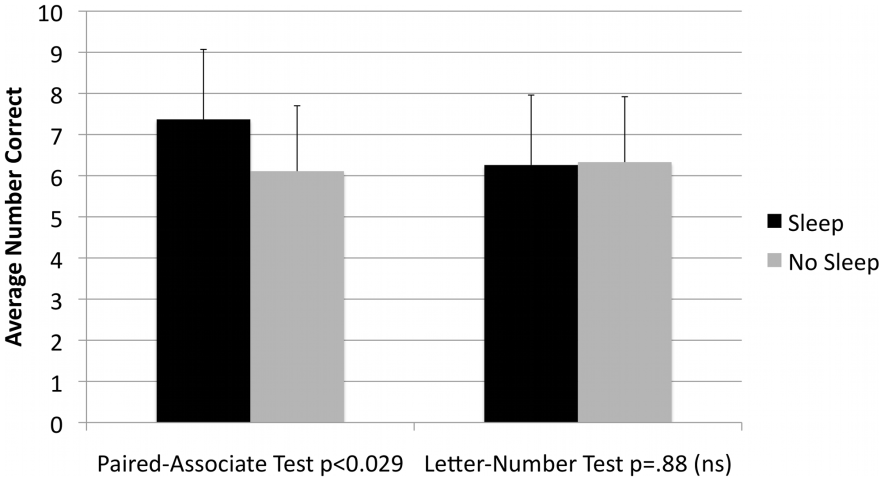
\includegraphics[width=\linewidth]{hypotheseGraph1}
	\caption{Conclusie studie Potkin en Bunney(2012)}
\end{figure}

Zoals je kan afleiden uit Figuur 1 verwachten we in week 1 dat mensen met een tekort aan slaap veel minder sterk zullen zijn in het opnemen van nieuwe informatie. Maar in week 2 verwachten we eigenlijk dat dit verschil iets minder groot zal zijn, dit omdat men reeds het onderwerp heeft ingestudeerd op een voorgaand moment en men de kennis dus al heeft, men moet het enkel nog reproduceren. Dit baseerden we op het artikel van \textcite{Potkin2012}.


\subsubsection{Hypothese omtrent muziek en Retrieval Practice}

\begin{figure}[H]
	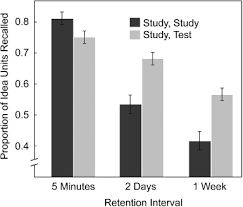
\includegraphics[width=0.8\linewidth]{hypotheseGraph2}
    \caption{Conclusie studie Roediger en Karpicke(2006)}
\end{figure}

In het algemeen verwachten we dat mensen die niet naar muziek luisteren beter gaan scoren. Dit gestaafd door het artikel van \textcite{Dolegui2013}.\\
\par
\noindent
In week 1 verwachten we dat het effect van Retrieval Practice nog niet echt zichtbaar zal zijn omdat de nadruk van deze studiemethode ligt op het langdurig beter onthouden van informatie en niet op het moment zelf dat men in aanraking komt ermee.
In week 2 verwachten we hier dus meer een onderscheid tussen. Omdat men nu enkel kennis moet reproduceren denken we dat muziek hier een kleiner effect zal hebben dan de invloed van Retrieval Practice, wat volgens ons zal uitblinken zoals je ook kan zien op de figuur. Dit denken we vooral door het originele artikel van \textcite{Roediger2006}.
\section{Data}

Welke data hebben we nu juist onderzocht? Wel, zoals voordien vermeld hebben we gekeken naar de verschillen tussen het niet of wel gebruiken van Retrieval Practice. Hierbij hebben we ook het effect van muziek toegevoegd. Verder hebben we ook een apart onderzoek gedaan waarbij we opzoek gingen naar het effect van de hoeveelheid slaap op de scores, losstaand van de andere variabelen.\\
\par
\noindent
Eerst en vooral hebben we een script geschreven in R om het effect van de hoeveelheid slaap te testen, hierbij hebben we drie verschillende intervallen gedefinieerd: 0 tot 5 uur slaap, 5 tot 8 uur slaap en meer dan 8 uur slaap.\\
\par
\noindent
Verder hebben we ook boxplots gemaakt waarin we de scores onderverdelen in 4 groepen: muziek luisteren, muziek luisteren met Retrieval Practice, enkel Retrieval Practice en alle overige situaties.

\section{Verklaringen}

\subsection{Hoeveelheid slaap}

\subsubsection{Het effect van slaap op het instuderen van de leerstof (week 1).}

\begin{figure}[H]
	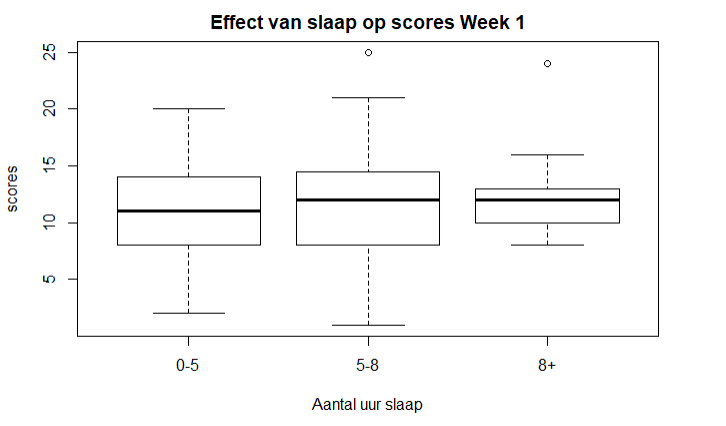
\includegraphics[width=\linewidth]{slaapGraph1}
    \caption{De invloed van slaap op scores in week 1}
\end{figure}


Hier kunnen we duidelijk zien dat slaap geen grote invloed heeft, maar er wel degelijk een invloed is. De gemiddelde scores van mensen met hoogstens 5 uur slaap liggen net iets lager dan de rest.

\subsubsection{Het effect van slaap op het behouden van de ingestudeerde leerstof (week 2).}

\begin{figure}[H]
	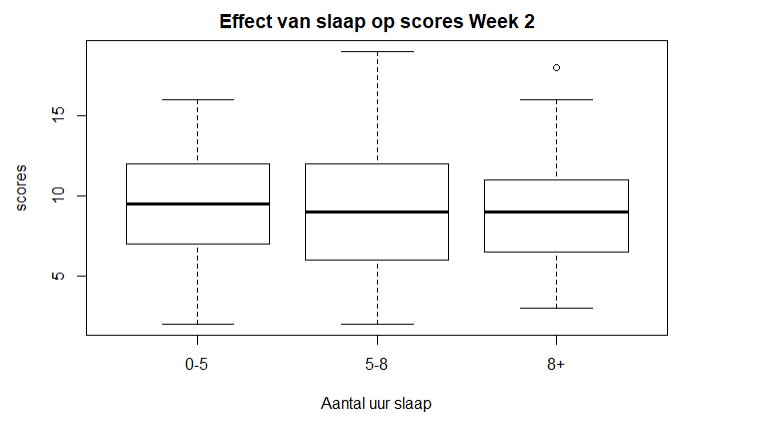
\includegraphics[width=\linewidth]{slaapGraph2}
    \caption{De invloed van slaap op scores in week 2}
\end{figure}

Bij de tweede week is dit verschil nog amper zichtbaar en scoren alle groepen ongeveer even goed.

\subsection{Retrieval Practice en het effect van muziek}

Deze werden zoals de voorgaande dataset ook geplot in R aan de hand van verschillende boxplots voor zowel week 1 als week 2.

\subsubsection{De mate waarin je leerstof voor korte termijn kunt instuderen (Week 1)}

\begin{figure}[H]
	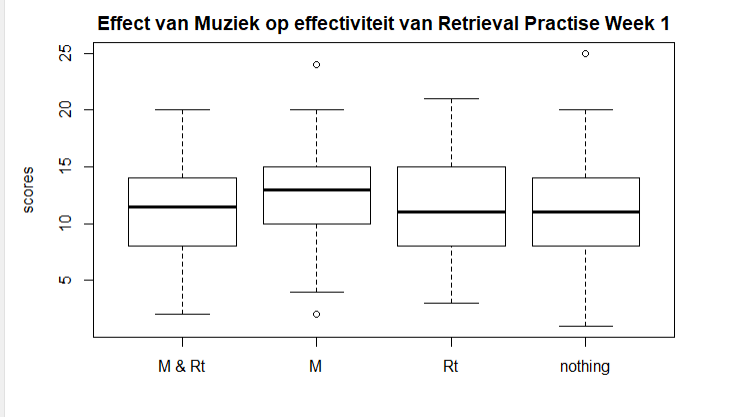
\includegraphics[width=\linewidth]{muziekGraph1}
    \caption{De invloed van muziek en Retrieval Practice in week 1}
\end{figure}

Hier bekijken we welke invloed zowel Retrieval Practice als muziek hebben op het instuderen van de leerstof.
\\
\begin{itemize}
    \item Eerst en vooral hebben we het gebruik van muziek tegenover geen muziek.
    Hieruit kunnen we verrassend genoeg toch afleiden dat muziek een positief effect lijkt te hebben op het instuderen van de leerstof, aangezien de scores voor mensen die muziek gebruikt hebben om het gevraagde in te studeren een hogere score hebben, al dan niet met retrieval practice of niet, dan mensen die niet naar muziek geluisterd hebben.
    \\
    \item Hierna bekijken we het verschil tussen Retrieval Practice tegenover geen Retrieval Practice.
    Hier ziet men in de eerste testweek geen verschil tussen het al dan niet gebruiken van Retrieval Practice, tot dusver komt dit dus nog overeen met het originele artikel \textcite{Roediger2006} waarop dit onderzoek gestaafd is.
    
\end{itemize}

\subsubsection{De mate waarin je kennis behoud op iets langere termijn (Week 2)}

\begin{figure}[H]
	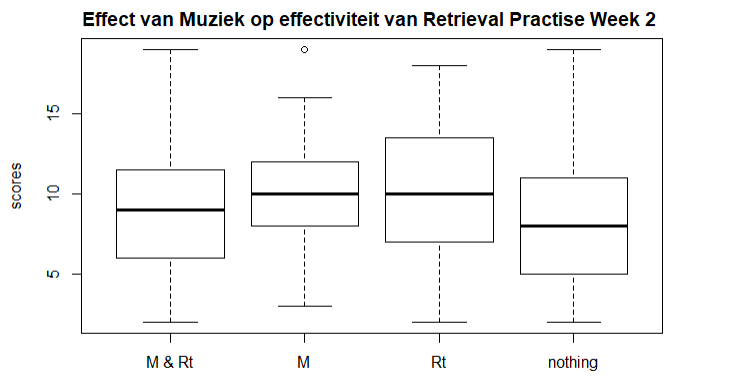
\includegraphics[width=\linewidth]{muziekGraph2}
    \caption{De invloed van muziek en Retrieval Practice in week 2}
\end{figure}

Als laatste bestuderen we de grafiek voor de tweede week en kijken we bij welke methodes je kunt zien dat er toch een groter behoud aan kennis is.\\

\begin{itemize}
    \item Het gebruik van muziek tegenover geen muziek: bij de tweede week is het “antwoord” toch niet meer zo eenduidig als het op muziek of geen muziek aankomt. Het verschil is aanzienlijk gezakt, wat toch blijk geeft dat indien men naar muziek luisterde in de eerste week men iets minder goed gememoriseerd heeft. Terwijl mensen die niet naar muziek luisteren wel net iets beter erin geslaagd zijn om hun kennis te behouden.
    \\
    \par
    \noindent
    Men ziet ook dat het al dan niet luisteren naar muziek niet echt een effect heeft op het oproepen van deze ingestudeerde kennis.
    \\
    \item Retrieval Practice tegenover geen Retrieval Practice: hier is er ondertussen wel een duidelijk verschil zichtbaar. Men ziet dat mensen die aan Retrieval Practice deden in de eerste week nu wel aanzienlijk beter hebben gescoord dan mensen die dit niet gedaan hebben. Dit met uitzondering van mensen die geen Retrieval Practice hebben toegepast maar wel naar muziek hebben geluisterd, die even goed scoren als de groep die retrieval practice heeft gebruikt. \\
    \par
    \noindent
    Hieruit kun je afleiden dat het al zeker beter is om aan Retrieval Practice te doen bij het studeren in plaats van de klassieke studiemethode, wat overeenkomt met het onderzoek van \textcite{Roediger2006}, maar dat het gebruik van enkel muziek (in dit geval klassieke muziek, ook wel Sedative Music genoemd zoals uitgelijnd in het artikel van \textcite{Dolegui2013}) ook geen nefast effect heeft op het behouden van eerder verworven kennis.
    
\end{itemize}
    

\section{Resultaten \& Conclusie }

Het doel van deze studie was om te kijken of Retrieval Practice wel degelijk een positieve invloed heeft op het onthouden van informatie (op lange termijn) en of muziek en een tekort aan slaap op hun beurt nadelige effecten hebben erop. In totaal waren er 240 deelnemers in het onderzoek. Elke deelnemer moest een tekst van ongeveer een anderhalve A4 pagina lang lezen en hiervan zoveel mogelijk informatie onthouden. De deelnemers werden initieel in 2 groepen verdeeld: een groep die aan Retrieval Practice deed (en de methode STST toepast) en een groep die gewoon op het einde pas een test deed (SSST). Vervolgens werden deze 2 groepen verder verveeld in enerzijds een groep die naar muziek (klassiek) luistert en anderzijds een groep die niet naar muziek luistert. Tot slot houden we ook rekening met het aantal uur dat iemand geslapen heeft.\\
\par
\noindent
Als we kijken naar de resultaten van het onderzoek zien we dat Retrieval Practice het veel beter doet dan de gewone klassieke studiemethode. Echter, de resultaten voor muziek en slaap zijn niet echt wat we verwacht hadden. Het verschil is gewoon te klein of het tegenovergestelde van wat we verwacht hadden/van de resultaten van de artikels waarop we ons onderzoek gebaseerd hebben. We denken dat dit door de kwaliteit van het onderzoek komt. De tekst was vrij kort en ging over iets waar de meeste mensen al (veel) kennis over hadden, we denken dus dat het iets te makkelijk was. Wat een verklaring is waarom de resultaten zo pover zijn. Ook zal het feit dat de deelnemers allemaal studenten waren voor dit vak, waarvan misschien een groot deel niet met alle positieve zin heeft deelgenomen, een invloed hebben. De verbetersleutel was volgens ons ook niet optimaal, er waren bijvoorbeeld 3 punten te verdienen met informatie over gemeenschappelijke voorouders die heel erg op elkaar leken (dit kon bijvoorbeeld samengenomen worden). Er was ook maar 1 week tussen de twee sessies, terwijl Retrieval Practice meer beloont als het over langere tijdsperioden gaat om informatie te onthouden. Als laatste vinden we ook dat de verbetering hier niet optimaal gedaan is, aangezien dit door zoveel verschillende mensen gebeurd is. Dit geeft verschillende perspectieven waardoor punten soms iets strenger of iets genereuzer bekomen konden worden. De verbetering is dus niet consistent.\\
\par
\noindent
Kortom, we zijn sterk van mening dat het onderzoek veel beter kon en dat de resultaten hiervan zeker niet beslissend zijn en met een korrel zout moeten genomen worden.

\section{Vervolgstudie en bedenkingen}
In onze eerste literatuurstudie hebben we het vooral gehad over het meten van de geheugencapaciteit van de testgroepen, en of er een correlatie is tussen de geheugencapaciteit en de doeltreffendheid van Retrieval Practice. Deze variabele hadden we toen opgenomen naar aanleiding van het artikel geschreven door \textcite{Agarwal2016}\\
\par
\noindent
Ook wilden we de retentietest hervormen volgens de principes van Rote Learning en Meaningful Learning (gebaseerd op het artikel van \textcite{Mayer2002}), om het effect van Retrieval Practice erop verder te bestuderen.
Concreet zouden we de proefpersonen opdelen in drie delen: Study-Study-Study-Study, Study-Study-Study-Test en Study-Test-Test-Test. Dit waren ook de omstandigheden van het origineel onderzoek door \textcite{Roediger2006} \\
\par
\noindent
Als hypotheses hadden we eerst dat Retrieval Practice een groter effect zou hebben bij mensen met een lage geheugencapaciteit, ten opzichte van mensen met een hogere geheugencapaciteit.  \\
Onze tweede hypothese was dat groepen die aan Rote Learning doen een beter resultaat zouden halen op de retentietest dan degene die het niet toepassen. 


%------------------------------------------------------------------------------
% Referentielijst
%------------------------------------------------------------------------------
% TODO: de gerefereerde werken moeten in BibTeX-bestand ``bibliografie.bib''
% voorkomen. Gebruik JabRef om je bibliografie bij te houden en vergeet niet
% om compatibiliteit met Biber/BibLaTeX aan te zetten (File > Switch to
% BibLaTeX mode)

\phantomsection
\printbibliography[heading=bibintoc]

\end{document}
